\documentclass[notes,serif]{beamer}
\usepackage{graphicx}
\usepackage{url}
\usepackage{clrscode}
\usepackage{amssymb,amsmath}

% You should run 'pdflatex' TWICE, because of TOC issues.

\mode<presentation>
{
  % A tip: pick a theme you like first, and THEN modify the color theme, and then add math content.
  % Warsaw is the theme selected by default in Beamer's installation sample files.

  %%%%%%%%%%%%%%%%%%%%%%%%%%%% THEME
  %\usetheme{AnnArbor}
  %\usetheme{Antibes}
  %\usetheme{Bergen}
  %\usetheme{Berkeley}
  %\usetheme{Berlin}
  %\usetheme{Boadilla}
  %\usetheme{boxes}
  %\usetheme{CambridgeUS}
  %\usetheme{Copenhagen}
  %\usetheme{Darmstadt}
  %\usetheme{default}
  %\usetheme{Dresden}
  %\usetheme{Frankfurt}
  %\usetheme{Goettingen}
  %\usetheme{Hannover}
  %\usetheme{Ilmenau}
  %\usetheme{JuanLesPins}
  %\usetheme{Luebeck}
  %\usetheme{Madrid}
  %\usetheme{Malmoe}
  %\usetheme{Marburg}
  %\usetheme{Montpellier}
  %\usetheme{PaloAlto}
  %\usetheme{Pittsburgh}
  %\usetheme{Rochester}
  %\usetheme{Singapore}
  %\usetheme{Szeged}
  \usetheme{Warsaw}

  %%%%%%%%%%%%%%%%%%%%%%%%%%%% COLOR THEME
  %\usecolortheme{albatross}
  %\usecolortheme{beetle}
  %\usecolortheme{crane}
  \usecolortheme{default}
  %\usecolortheme{dolphin}
  %\usecolortheme{dove}
  %\usecolortheme{fly}
  %\usecolortheme{lily}
  %\usecolortheme{orchid}
  %\usecolortheme{rose}
  %\usecolortheme{seagull}
  %\usecolortheme{seahorse}
  %\usecolortheme{sidebartab}
  %\usecolortheme{structure}
  %\usecolortheme{whale}

  %%%%%%%%%%%%%%%%%%%%%%%%%%%% OUTER THEME
  %\useoutertheme{default}
  %\useoutertheme{infolines}
  %\useoutertheme{miniframes}
  %\useoutertheme{shadow}
  %\useoutertheme{sidebar}
  %\useoutertheme{smoothbars}
  %\useoutertheme{smoothtree}
  %\useoutertheme{split}
  %\useoutertheme{tree}

  %%%%%%%%%%%%%%%%%%%%%%%%%%%% INNER THEME
  %\useinnertheme{circles}
  %\useinnertheme{default}
  %\useinnertheme{inmargin}
  %\useinnertheme{rectangles}
  %\useinnertheme{rounded}

  %%%%%%%%%%%%%%%%%%%%%%%%%%%%%%%%%%%

%  \setbeamercovered{transparent} % or whatever (possibly just delete it)
  \setbeamercovered{invisible} % or whatever (possibly just delete it)
  % To change behavior of \uncover from graying out to totally invisible, can change \setbeamercovered to invisible instead of transparent. apparently there are also 'dynamic' modes that make the amount of graying depend on how long it'll take until the thing is uncovered.

}


% Get rid of nav bar
\beamertemplatenavigationsymbolsempty

% Use short top
%\usepackage[headheight=12pt,footheight=12pt]{beamerthemeboxes}
%\addheadboxtemplate{\color{black}}{
%\hskip0.3cm
%\color{white}
%\insertshortauthor \ \ \ \
%\insertframenumber \ \ \ \ \ \ \
%\insertsection \ \ \ \ \ \ \ \ \ \ \ \ \ \ \ \ \  \insertsubsection
%\hskip0.3cm}
%\addheadboxtemplate{\color{black}}{
%\color{white}
%\ \ \ \
%\insertsection
%}
%\addheadboxtemplate{\color{black}}{
%\color{white}
%\ \ \ \
%\insertsubsection
%}

% Insert frame number at bottom of the page.
\usefoottemplate{\hfil\tiny{\color{black!90}\insertframenumber}}

\usepackage[english]{babel}
\usepackage[latin1]{inputenc}

\usepackage{times}
\usepackage[T1]{fontenc}

\title{Network Programming}
\subtitle{Lecture 6---Advanced Sockets II: \\ Routing Sockets, Key Management Sockets, and Threads}

\author{Lei Wang\\ lei.wang@dlut.edu.cn}

\institute{Dalian University of Technology}

\date{Dec 22, 2008}

\subject{Talks}

\def\defn#1{{\color{red} #1}}

\begin{document}

\begin{frame}
  \titlepage
\end{frame}

\begin{frame}
  \frametitle{Part 3. Advanced Sockets II: \\ Routing Sockets, Key Management Sockets, and Threads}
  \tableofcontents
\end{frame}

\begin{frame}
  \frametitle{}
  \begin{block}{}
    \begin{center}
    {\Large Chapter 18: Routing Sockets}      
    \end{center}
  \end{block}
\end{frame}

\section{Routing Sockets}
\subsection{Introduction}
\begin{frame}
  \frametitle{Routing Sockets Introduction}
  \texttt{AF\_ROUTE} domain: The only type of socket is \textbf{raw socket}.  Three types of operations supported on a routing socket:
  \begin{itemize}
    \item A process can send a message to the kernel by writing to a routing socket. (e.g. add and delete route)
    \item A process can read a message from the kernel on a routing socket.  (e.g. kernel notify a process that an ICMP redirect has been received)
    \item A process can use the \texttt{sysctl} function to either dump the routing table or list all configured interfaces.
  \end{itemize}
\end{frame}

\subsection{Datalink Socket Address Structures}
\begin{frame}[containsverbatim]
  \frametitle{Datalink Socket Address Structures}
  {\tiny
  \begin{verbatim}
struct sockaddr_dl {
  uint8_t      sdl_len;
  sa_family_t  sdl_family;   /* AF_LINK */
  uint16_t     sdl_index;    /* system assigned index, if > 0 */
  uint8_t      sdl_type;     /* IFT_ETHER, etc. from <net/if_types.h> */
  uint8_t      sdl_nlen;     /* name length, starting in sdl_data[0] */
  uint8_t      sdl_alen;     /* link-layer address length */
  uint8_t      sdl_slen;     /* link-layer selector length */
  char         sdl_data[12]; /* minimum work area, can be larger;
                                contains i/f name and link-layer address */
};
  \end{verbatim}
  }
\end{frame}

\subsection{Reading and Writing}
\begin{frame}
  \frametitle{Reading and Writing}
  \begin{figure}
    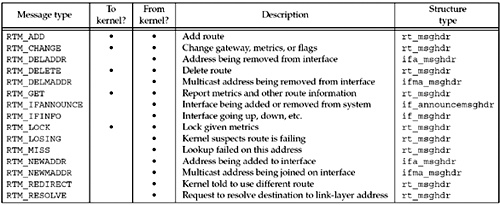
\includegraphics[width=.7\textwidth]{figs/18fig02}
    \caption{18.2 Types of messages exchanged across a routing socket.}
  \end{figure}
\end{frame}

\begin{frame}
  \frametitle{Example: Fetch and Print a Routing Table Entry}
  \begin{itemize}
    \item \texttt{route/getrt.c}
  \end{itemize}
\end{frame}

\begin{frame}
  \frametitle{}
  \begin{block}{}
    \begin{center}
    {\Large Chapter 19: Key Management Sockets}      
    \end{center}
  \end{block}
\end{frame}
\section{Key Management Sockets}
\subsection{Introduction}
\begin{frame}
  \frametitle{Key Management Sockets Introduction}
  IPsec needs a mechanism to manage secret encryption and authorization keys.  RFC 2367 introduces a generic key management API for IPsec and other security services.
\begin{itemize}
  \item New protocol family: \texttt{PF\_KEY}: only type of socket supported in this domain is a raw socket.
  \item Superuser privilege required.
  \item SA (Security Association) and SADB (Security Association database)
  \item More than one SA can apply to a single stream of traffic.
  \item SADB may be used for more than just IPsec; e.g. OSPFv2, RIPv2, so \texttt{PF\_KEY} sockets are not specific to IPsec.
\end{itemize}
\end{frame}

\subsection{Reading and Writing}
\begin{frame}[containsverbatim]
  \frametitle{Key Management Message Header}
  {\scriptsize
  \begin{verbatim}
struct sadb_msg {
 u_int8_t sadb_msg_version;   /* PF_KEY_V2 */
 u_int8_t sadb_msg_type;      /* see Figure 19.2 */
 u_int8_t sadb_msg_errno;     /* error indication */
 u_int8_t sadb_msg_satype;    /* see Figure 19.3 */
 u_int16_t sadb_msg_len;      /* length of header + extensions / 8 */
 u_int16_t sadb_msg_reserved; /* 0 on transmit, ignored on receive */
 u_int32_t sadb_msg_seq;      /* sequence number */
 u_int32_t sadb_msg_pid;      /* process ID of source or dest */
};
  \end{verbatim}
  }
\end{frame}

\begin{frame}
  \frametitle{Type of Messages}
  \begin{figure}
    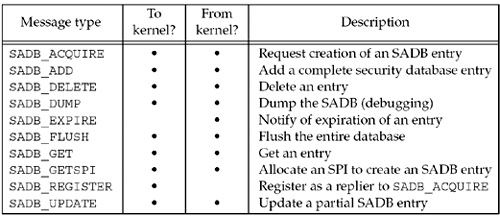
\includegraphics[width=.7\textwidth]{figs/19fig02}
    \caption{19.2 Types of messages exchanged across a \texttt{PF\_KEY} socket}
  \end{figure}
\end{frame}

\begin{frame}
  \frametitle{Types of SAs}
  \begin{figure}
    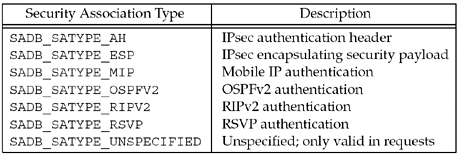
\includegraphics[width=.7\textwidth]{figs/19fig03}
    \caption{19.3 Types of SAs}
  \end{figure}
\end{frame}

\subsection{Example: Dumping the Security Association Database}
\begin{frame}
  \frametitle{Example: Dumping the Security Association Database}
\begin{itemize}
  \item \texttt{key/dump.c}
\end{itemize}
\end{frame}

\begin{frame}[containsverbatim]
  \frametitle{Creating a Static Security Association}
  SA Extensions:
  {\scriptsize
  \begin{verbatim}
struct sadb_sa {
  u_int16_t sadb_sa_len;      /* length of extension / 8 */
  u_int16_t sadb_sa_exttype;  /* SADB_EXT_SA */
  u_int32_t sadb_sa_spi;      /* Security Parameters Index (SPI) */
  u_int8_t  sadb_sa_replay;   /* replay window size, or zero */
  u_int8_t  sadb_sa_state;    /* SA state, see Figure 19.7 */
  u_int8_t  sadb_sa_auth;     /* authentication algorithm, see Figure 19.8 */
  u_int8_t  sadb_sa_encrypt;  /* encryption algorithm, see Figure 19.8 */
  u_int32_t sadb_sa_flags;    /* bitmask of flags */
};
  \end{verbatim}
  }
\end{frame}

\begin{frame}[containsverbatim]
  \frametitle{Dynamically Maintaining SAs}
  {\scriptsize
  \begin{itemize}
    \item A daemon registers itself with the kernel using the \texttt{SADB\_REGISTER} message, specifying the type of SA it can handle in the \texttt{sadb\_msg\_satype}.
    \item If a daemon can handle multiple SA types, it sends multiple \texttt{SADB\_REGISTER} messages, each registering a single type.
    \item In the \texttt{SADB\_REGISTER} reply message, the kernel includes a supported algorithms extension, indicating what encryption and/or authentication mechanisms are supported (by an \texttt{sadb\_supported} structure).
  \end{itemize}
  }
  {\tiny
  \begin{verbatim}
struct sadb_supported {
  u_int16_t sadb_supported_len;      /* length of extension + algorithms / 8 */
  u_int16_t sadb_supported_exttype;  /* SADB_EXT_SUPPORTED_{AUTH, ENCRYPT} */
  u_int32_t sadb_supported_reserved; /* reserved for future expansion */
};
                                     /* followed by algorithm list */

struct sadb_alg {
  u_int8_t sadb_alg_id;              /* algorithm ID from Figure 19.8 */
  u_int8_t sadb_alg_ivlen;           /* IV length, or zero */
  u_int16_t sadb_alg_minbits;        /* minimum key length */
  u_int16_t sadb_alg_maxbits;        /* maximum key length */
  u_int16_t sadb_alg_reserved;       /* reserved for future expansion */
};
  \end{verbatim}
  }
\end{frame}



\begin{frame}
  \frametitle{}
  \begin{block}{}
    \begin{center}
    {\Large Chapter 26: Threads}      
    \end{center}
  \end{block}
\end{frame}

\section{Threads}
\subsection{Thread Introduction}
\begin{frame}
  \frametitle{Thread Introduction}
  Unix traditional process paradigm: \texttt{fork} new processes, but there are problems with \texttt{fork}:
  \begin{itemize}
    \item \texttt{fork} is expensive.  Memory is copied from the parent to the child, all descriptors are duplicated in the child, and so on.
    \item IPC is required to pass information between the parent and child after the \texttt{fork}.  Parent to child is easy, but not the case vice versa.
  \end{itemize}
  Threads help with both problems:
  \begin{itemize}
    \item \textit{lightweight processes}---``lighter weight'' than a process: 10--100 times faster
    \item All threads within a process share the same global memory---sharing is easy, \textbf{but} along with this simplicity comes the problem of \textit{synchronization}.
  \end{itemize}
\end{frame}

\begin{frame}
  \frametitle{Thread Introduction contd.}
  \begin{exampleblock}{Shared}
    {
    \small
    All threads within a process share the following:
  \begin{itemize}
    \item Global variables
    \item Process instructions
    \item Most data
    \item Open files (e.g. descriptors)
    \item Signal handlers and signal dispositions
    \item Current working directory
    \item User and group IDs
  \end{itemize}
  }
  \end{exampleblock}

\end{frame}

\begin{frame}
  \frametitle{Thread Introduction contd.}
  \begin{alertblock}{Its own}
    {
    \small
    All threads within a process share the following:
  \begin{itemize}
    \item Thread ID
    \item Set of registers, including program counter and stack pointer
    \item Stack (for local variables and return addresses)
    \item \texttt{errno}
    \item Signal mask
    \item Priority
  \end{itemize}
  One analogy is to think of signal handlers as a type of thread, i.e. the main flow of execution (one thread) and a signal handler (another thread); both threads share the same global variables, but each has its own stack.
  }
  \end{alertblock}
\end{frame}

\subsection{Basic Functions: Creation and Termination}
\begin{frame}[containsverbatim]
  \frametitle{Basic Functions: Creation and Termination}
  \begin{itemize}
    \item \texttt{pthread\_create} Function \\
      {\scriptsize
      \verb+int pthread_create(pthread_t *tid, const pthread_attr_t *attr,+
      \verb+                       void *(*func) (void *), void *arg);+
      }
    \item \texttt{pthread\_join} Function \\
      {\scriptsize
      \verb+int pthread_join(pthread_t tid, void ** status);+
      }
    \item \texttt{pthread\_self} Function \\
      {\scriptsize
      \verb+pthread_t pthread_self(void);+
      }
    \item \texttt{pthread\_detach} Function \\
      {\scriptsize
      \verb+int pthread_detach(pthread_t tid);+
      }
    \item \texttt{pthread\_exit} Function \\
      {\scriptsize
      \verb+oid pthread_exit (void *status);+
      }
  \end{itemize}
  All functions defined in \verb+<pthread.h>+
\end{frame}

\subsection{Example: \texttt{str\_cli} Function and TCP Echo Server}
\begin{frame}
  \frametitle{Example: \texttt{str\_cli} Function and TCP Echo}
  \begin{itemize}
    \item \texttt{threads/strclithread.c} \\
      \begin{figure}
        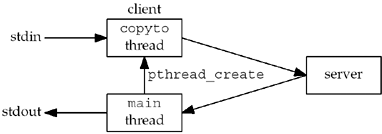
\includegraphics[width=.5\textwidth]{figs/26fig01}
        \caption{26.1 Recoding \texttt{str\_cli} to use threads.}
      \end{figure}
    \item \texttt{threads/tcpserv01.c}
  \end{itemize}
\end{frame}

\subsection{Mutexes: Mutual Exclusion}
\begin{frame}[containsverbatim]
  \frametitle{Mutexes: Mutual Exclusion}
  \begin{itemize}
    \item A typical problem with \textit{concurrent programming} or \textit{parallel programming}
    \item In terms of Pthreads, it is a variable of type \texttt{pthread\_metex\_t}, used with the following two functions: \\
        {\scriptsize
      \verb+int pthread_mutex_lock(pthread_mutex_t * mptr);+
      \verb+int pthread_mutex_unlock(pthread_mutex_t * mptr);+
      }
  \end{itemize}
\end{frame}

\subsection{Condition Variables}
\begin{frame}[containsverbatim]
  \frametitle{Condition Variables}
  \begin{itemize}
    \item We need something to let us go to sleep waiting for some condition to occur.
    \item Mutex provides mutual exclusion and the condition variable provides a signaling mechanism.
    \item In terms of Pthreads, it is a variable of type \texttt{pthread\_cond\_t}, used with the following two functions: \\
        {\tiny
      \verb+int pthread_cond_wait(pthread_cond_t *cptr, pthread_mutex_t *mptr);+
      \verb+int pthread_cond_signal(pthread_cond_t *cptr);+
      }
  \end{itemize}
\end{frame}

\begin{frame}
  \frametitle{Summary}
  \begin{itemize}
    \item Creation of threads are normally faster than creation of a new process with \texttt{fork}.
    \item All threads in a process share global variables and descriptors.  (Cause synchronization problems, so mutexes and condition variables)
    \item Thread safe issue.
  \end{itemize}
\end{frame}

\end{document}
